
\begin{figure}[t!]
\centering
\begin{minipage}[t]{0.44\textwidth}
 %   \subfloat[]{
     \resizebox {\columnwidth} {!} {
        \begin{tikzpicture}
        \pgfplotsset{every axis legend/.append style={
at={(0.5,1.03)},
anchor=south}}

        % LEFT AXIS
        % =========
        \begin{axis}[
          enlargelimits=false,
          ylabel={\large  Seen Acc. (\%)},
          xlabel={},
           xmin=0, xmax=72,
           ymin=22, ymax=53,
          xtick={0,8,16,32,48,64},
          ytick={20,25,30,35,40,45,50},
          %legend pos=south west,
          ymajorgrids=true,
          grid style=dashed,
          width=10cm,
          height=4.5cm,
          legend columns=2,
        legend style={draw=none},
        every axis plot/.append style={ultra thick},
        every mark/.append style={mark size=50pt}
        ]
        
        \addplot[
          color=MaterialBlue800,
          mark=square*]
        table[x index=0,y index=1,col sep=comma]
        {tex/Tables/Tab/seen-clean-static-i3d.txt};
               \addlegendentry{I3D-(with clean)} 
         
        
        
        % An \addplot for each line
        \addplot[
          color=MaterialOrange800,
          mark=oplus*]
        table[x index=0,y index=1,col sep=comma]
        {tex/Tables/Tab/seen-clean-static-MoViNet.txt};
       \addlegendentry{MoViNet-(with clean)} 
       
       %%%%%%%%%%%%%%%%%%%%
       %  no clean buffer %
       %%%%%%%%%%%%%%%%%%%%
       
        \addplot[dotted,
          color=MaterialBlue800,]
        table[x index=0,y index=1,col sep=comma]
        {tex/Tables/Tab/seen-noclean-i3d.txt};
               \addlegendentry{I3D-(w/o clean)} 
         
        
        
        % An \addplot for each line
        \addplot[dotted,
          color=MaterialOrange800,]
        table[x index=0,y index=1,col sep=comma]
        {tex/Tables/Tab/seen-noclean-MoViNet.txt};
       \addlegendentry{MoViNet-(w/o clean)} 


        \end{axis}
        
        \end{tikzpicture}%
      }

    \end{minipage}
\begin{minipage}[t]{0.44\textwidth}
 %   \subfloat[]{
     \resizebox {\columnwidth} {!} {
        \begin{tikzpicture}
        \pgfplotsset{every axis legend/.append style={
at={(0.5,1.03)},
anchor=south}}

        % LEFT AXIS
        % =========
        \begin{axis}[
          enlargelimits=false,
          ylabel={\large Unseen Acc. (\%)},
          xlabel={},
           xmin=0, xmax=72,
           ymin=20, ymax=37,
          xtick={0,8,16,32,48,64},
          ytick={22,24,28,30,32,34},
          %legend pos=south west,
          ymajorgrids=true,
          grid style=dashed,
          width=10cm,
          height=4.5cm,
          legend columns=2,
        legend style={draw=none},
        every axis plot/.append style={ultra thick},
        every mark/.append style={mark size=50pt}
        ]
        
        \addplot[
          color=MaterialBlue800,
          mark=square*]
        table[x index=0,y index=1,col sep=comma]
        {tex/Tables/Tab/unseen-clean-static-i3d.txt};
               \addlegendentry{I3D-(with clean)} 

         
       % \addlegendentry{Single-DG-RNA} 
        
        
        % An \addplot for each line
        \addplot[
          color=MaterialOrange800,
          mark=oplus*]
        table[x index=0,y index=1,col sep=comma]
        {tex/Tables/Tab/unseen-clean-static-MoViNet.txt};
       \addlegendentry{MoViNet-(with clean)} 
        
        
       %%%%%%%%%%%%%%%%%%%%
       %  no clean buffer %
       %%%%%%%%%%%%%%%%%%%%
       
        \addplot[dotted,
          color=MaterialBlue800,]
        table[x index=0,y index=1,col sep=comma]
        {tex/Tables/Tab/unseen-noclean-i3d.txt};
               \addlegendentry{I3D-(w/o clean)} 
         
        
        
        % An \addplot for each line
        \addplot[dotted,
          color=MaterialOrange800,]
        table[x index=0,y index=1,col sep=comma]
        {tex/Tables/Tab/unseen-noclean-MoViNet.txt};
       \addlegendentry{MoViNet-(w/o clean)} 
        
        \end{axis}  
        
        \end{tikzpicture}%
      }

    \end{minipage}
%%%%%%%%%%%%%
%   graph   %
%%%%%%%%%%%%%

%\begin{minipage}[t]{0.44\textwidth}
 %   \subfloat[]{
%    \resizebox {\columnwidth} {!}{
%    \centering
%    %%%%%%%%%%%%%%%%%%%%%%%%%%%%%%%%%%%%%%%%%%%%%%%%%%%%%%%%%%%%%%%
%
% Welcome to Overleaf --- just edit your LaTeX on the left,
% and we'll compile it for you on the right. If you open the
% 'Share' menu, you can invite other users to edit at the same
% time. See www.overleaf.com/learn for more info. Enjoy!
%
%%%%%%%%%%%%%%%%%%%%%%%%%%%%%%%%%%%%%%%%%%%%%%%%%%%%%%%%%%%%%%%
%\usepgfplotslibrary{external}
%\tikzexternalize

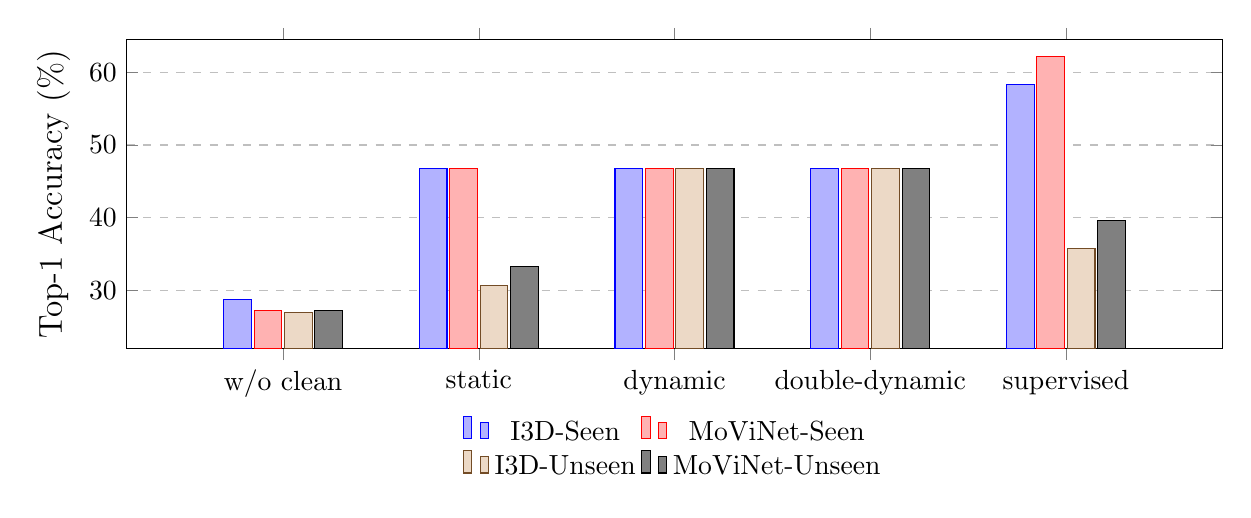
\begin{tikzpicture}
\centering
\begin{axis}[
symbolic x coords={w/o clean, static, dynamic, double-dynamic, supervised},
	ylabel=\large Top-1 Accuracy (\%),
	enlargelimits=false,
	ybar=1pt, enlarge x limits=0.2,
	xtick=data,
	ymin=22.0,
    ymax=64.5,
    ymajorgrids=true,
    legend style={draw=none},
          grid style=dashed,
          width=15.5cm,
          height=5.5cm,
         legend style={at={(0.5,-0.2)},
	    anchor=north,legend columns=2}, 
        every axis plot/.append 
        every mark/.append style={mark size=52pt}
]
\addplot 
	coordinates {(w/o clean,28.73) (static,46.77) (dynamic,46.77) (double-dynamic,46.77)
	(supervised,58.33) };
	\addlegendentry{I3D-Seen} 
\addplot 
	coordinates {(w/o clean,27.20) (static,46.71) (dynamic,46.71)(double-dynamic,46.77)
	(supervised,62.24) };
	\addlegendentry{MoViNet-Seen} 
\addplot 
	coordinates {(w/o clean,26.96) (static,30.71) (dynamic,46.71)(double-dynamic,46.77)
	(supervised,35.71) };
\addlegendentry{I3D-Unseen} 
\addplot 
	coordinates {(w/o clean,27.20) (static,33.30) (dynamic,46.71)(double-dynamic,46.77)
	(supervised,39.59) };
\addlegendentry{MoViNet-Unseen} 

\end{axis}
\end{tikzpicture}



%    }
%    \vspace{0.4cm}
%    \end{minipage}    


%%%%%%%%%%%%%%
%   graph 2  %
%%%%%%%%%%%%%%
%\begin{minipage}[t]{0.44\textwidth}
% %   \subfloat[]{
%    \resizebox {\columnwidth} {!}{
%    \centering
%    %%%%%%%%%%%%%%%%%%%%%%%%%%%%%%%%%%%%%%%%%%%%%%%%%%%%%%%%%%%%%%%
%
% Welcome to Overleaf --- just edit your LaTeX on the left,
% and we'll compile it for you on the right. If you open the
% 'Share' menu, you can invite other users to edit at the same
% time. See www.overleaf.com/learn for more info. Enjoy!
%
%%%%%%%%%%%%%%%%%%%%%%%%%%%%%%%%%%%%%%%%%%%%%%%%%%%%%%%%%%%%%%%
%\usepgfplotslibrary{external}
%\tikzexternalize

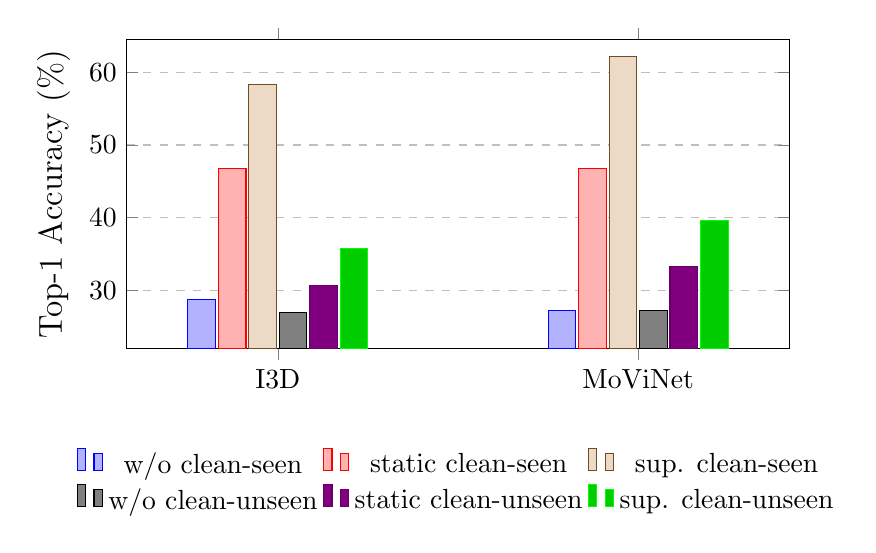
\begin{tikzpicture}
\begin{axis}[
symbolic x coords={I3D, MoViNet},
	ylabel=\large Top-1 Accuracy (\%),
	enlargelimits=false,
	ybar=1pt, enlarge x limits=0.42,
	xtick=data,
	ymin=22.0,
    ymax=64.5,
    ymajorgrids=true,
    legend style={draw=none},
          grid style=dashed,
          width=10cm,
          height=5.5cm,
         legend style={at={(0.5,-0.3)},
	    anchor=north,legend columns=3}, 
        every axis plot/.append 
        every mark/.append style={mark size=52pt}
]
\addplot 
	coordinates {
	            (I3D,28.73)
	            (MoViNet,27.20)
	};
	\addlegendentry{w/o clean-seen} 
\addplot 
	coordinates {
	            (I3D,46.77)
	            (MoViNet,46.71)
	};
	\addlegendentry{static clean-seen} 
\addplot 
	coordinates {
	            (I3D,58.33)
	            (MoViNet,62.24)
	};
	\addlegendentry{sup. clean-seen} 
	
	
	

\addplot 
	coordinates {
	            (I3D,26.96)
	            (MoViNet,27.20)
	};
	\addlegendentry{w/o clean-unseen} 

\addplot 
	coordinates {
	            (I3D,30.71)
	            (MoViNet,33.30)
	};
	\addlegendentry{static clean-unseen} 

\addplot 
	coordinates {
	            (I3D,35.71)
	            (MoViNet,39.59)
	};
	\addlegendentry{sup. clean-unseen} 

\end{axis}
\end{tikzpicture}



%    }
%    
%    \end{minipage}    
        
    

\caption{\textbf{Static boundary localization.} Top-1 \textit{mean} accuracy ($\%$), over all $D_i \rightarrow D_j$ combinations on both seen (up) and unseen (down) test sets in \textit{online-trimmed} setting, with different clean buffer strategy w.r.t the no-clean buffer. }
\label{fig:clean_static}
\end{figure}